\documentclass[12pt]{article}

\usepackage{amsmath, mathtools}
\usepackage{amsfonts}
\usepackage{amssymb}
\usepackage{graphicx}
\usepackage{colortbl}
\usepackage{xr}
\usepackage{hyperref}
\usepackage{longtable}
\usepackage{xfrac}
\usepackage{tabularx}
\usepackage{float}
\usepackage{siunitx}
\usepackage{booktabs}
\usepackage{caption}
\usepackage{pdflscape}
\usepackage{afterpage}

\usepackage[round]{natbib}

%\usepackage{refcheck}

\hypersetup{
    bookmarks=true,         % show bookmarks bar?
      colorlinks=true,       % false: boxed links; true: colored links
    linkcolor=black,          % color of internal links (change box color with 
    %linkbordercolor)
    citecolor=blue,        % color of links to bibliography
    filecolor=magenta,      % color of file links
    urlcolor=cyan           % color of external links
}

%% Comments

\usepackage{color}

\newif\ifcomments\commentstrue

\ifcomments
\newcommand{\authornote}[3]{\textcolor{#1}{[#3 ---#2]}}
\newcommand{\todo}[1]{\textcolor{red}{[TODO: #1]}}
\else
\newcommand{\authornote}[3]{}
\newcommand{\todo}[1]{}
\fi

\newcommand{\wss}[1]{\authornote{blue}{SS}{#1}}
\newcommand{\hz}[1]{\authornote{magenta}{Author}{#1}}


% For easy change of table widths
\newcommand{\colZwidth}{1.0\textwidth}
\newcommand{\colAwidth}{0.13\textwidth}
\newcommand{\colBwidth}{0.82\textwidth}
\newcommand{\colCwidth}{0.1\textwidth}
\newcommand{\colDwidth}{0.05\textwidth}
\newcommand{\colEwidth}{0.8\textwidth}
\newcommand{\colFwidth}{0.17\textwidth}
\newcommand{\colGwidth}{0.5\textwidth}
\newcommand{\colHwidth}{0.28\textwidth}

% Used so that cross-references have a meaningful prefix
\newcounter{defnum} %Definition Number
\newcommand{\dthedefnum}{GD\thedefnum}
\newcommand{\dref}[1]{GD\ref{#1}}
\newcounter{datadefnum} %Datadefinition Number
\newcommand{\ddthedatadefnum}{DD\thedatadefnum}
\newcommand{\ddref}[1]{DD\ref{#1}}
\newcounter{theorynum} %Theory Number
\newcommand{\tthetheorynum}{T\thetheorynum}
\newcommand{\tref}[1]{T\ref{#1}}
\newcounter{tablenum} %Table Number
\newcommand{\tbthetablenum}{T\thetablenum}
\newcommand{\tbref}[1]{TB\ref{#1}}
\newcounter{assumpnum} %Assumption Number
\newcommand{\atheassumpnum}{P\theassumpnum}
\newcommand{\aref}[1]{A\ref{#1}}
\newcounter{calcnum} %Calculation number
\newcommand{\cthecalcnum}{C\thecalcnum}
\newcommand{\calcref}[1]{C\ref{#1}}
\newcounter{goalnum} %Goal Number
\newcommand{\gthegoalnum}{P\thegoalnum}
\newcommand{\gsref}[1]{GS\ref{#1}}
\newcounter{instnum} %Instance Number
\newcommand{\itheinstnum}{IM\theinstnum}
\newcommand{\iref}[1]{IM\ref{#1}}
\newcounter{reqnum} %Requirement Number
\newcommand{\rthereqnum}{P\thereqnum}
\newcommand{\rref}[1]{R\ref{#1}}
\newcounter{nfreqnum} %Nonfunctional Requirement Number
\newcommand{\rthenfreqnum}{P\thenfreqnum}
\newcommand{\nfrref}[1]{NFR\ref{#1}}
\newcounter{lcnum} %Likely change number
\newcommand{\lthelcnum}{LC\thelcnum}
\newcommand{\lcref}[1]{LC\ref{#1}}
\newcommand\inn{ %math element of symbol
	\mathrel{\ooalign{$\subset$\cr\hfil\scalebox{0.8}[1]{$=$}\hfil\cr}}%
}
\newcommand{\famname}{LoSMS} % PUT YOUR PROGRAM NAME 
%HERE

\usepackage{fullpage}

\begin{document}

\title{A Library of Simplex Method Solvers} 
\author{Hanane Zlitni}
\date{October 4, 2018}

\maketitle

~\newpage

\pagenumbering{roman}

\section{Revision History}

\begin{tabularx}{\textwidth}{p{3cm}p{2cm}X}
	\toprule {\bf Date} & {\bf Version} & {\bf Notes}\\
	\midrule
	October 4, 2018 & 1.0 & First Draft\\
	\bottomrule
\end{tabularx}

~\newpage
	
\section{Reference Material}

This section records information for easy reference.

\subsection{Table of Units}

This section is not applicable for \famname{}.

\subsection{Table of Symbols}

The table that follows summarizes the symbols used in this document.

\renewcommand{\arraystretch}{1.2}
%\noindent \begin{tabularx}{1.0\textwidth}{l l X}
\noindent \begin{longtable*}{l l p{12cm}} \toprule
\textbf{symbol} & \textbf{unit} & \textbf{description}\\
\midrule 
	$Z$ & - & Optimal solution of the objective function\\
\bottomrule
\end{longtable*}

\subsection{Abbreviations and Acronyms}

\renewcommand{\arraystretch}{1.2}
\begin{tabular}{l l} 
  \toprule		
  \textbf{symbol} & \textbf{description}\\
  \midrule 
  A & Assumption\\
  C & Calculation \\
  DD & Data Definition\\
  GD & General Definition\\
  GS & Goal Statement\\
  IM & Instance Model\\
  LC & Likely Change\\
  PS & Physical System Description\\
  R & Requirement\\
  SRS & Software Requirements Specification\\
  CA & Commonality Analysis\\
  \famname{} & Library of Simplex Method Solvers\\
  T & Theoretical Model\\
  s.t. & Subject to\\
  \bottomrule
\end{tabular}\\

\newpage

\tableofcontents

~\newpage

\pagenumbering{arabic}

\section{Introduction}

The simplex method, a linear programming algorithm, is considered one of the 
most popular algorithms that has significant influence in the fields of science 
and engineering (\cite{simplex-popularity}). 

The algorithm can be used in a variety of fields and its goal is to make the 
most of the available resources to achieve the optimal solution. For example, 
the simplex method is used in the sand casting process to optimize the sand 
casting parameters to produce the best results (\cite{sand-casting}). Moreover, 
the simplex method was used in chemistry to maximize the yield of a chemical 
reaction (\cite{chemistry}).

Since the simplex method has various applications in different fields, a 
software that facilitates solving objective functions using the simplex method 
for different purposes can be useful. 

This commonality analysis (CA) provides detailed documentation of a 
general-purpose program family, called \famname{}, that solves linear 
programming problems using the simplex method. The CA template is based on 
\citet{Smith2006}.

\subsection{Purpose of Document}

The purpose of this document is to formally describe the requirements for the 
development of the \famname{} tool which simplifies obtaining the optimal 
solution of linear programs. Having a thorough and comprehensive documentation 
of this tool would be useful for future use of \famname{}, possible 
enhancements and maintenance.

\subsection{Scope of the Family} 

The scope of \famname{} is limited to solving linear equations using the 
simplex method. The tool supports both maximization and minimization linear 
programs.

\subsection{Characteristics of Intended Reader} 

The intended reader of this document must have basic knowledge of linear 
programming which is typically given to year 3 undergraduate students. The 
intended reader must also have basic knowledge of linear algebra and calculus. 
No technical background is required.

\subsection{Organization of Document}

The document begins by providing a general description of the system, which 
includes potential system contexts, user characteristics and system 
constraints, in Section \ref{SecSystemDescription}. Then, Section 
\ref{Sec_Commonalities} describes the commonalities in the \famname{} program 
family by giving a background overview of the tool, terminology definitions, 
data definitions that are used to build instance models, goal statements and 
theoretical models. Next, Section \ref{Sec_Variabilities} details the 
variabilities in the tool and consists of instance models and assumptions. This 
is followed by the functional and nonfunctional requirements of the \famname{} 
tool in Section \ref{Sec_Requirements} and likely changes in variabilities in 
Section \ref{Sec_LikelyChanges}. Finally, Section \ref{Sec_TraceabilityMatrix} 
visualises the way different sections of this document can be traced to one 
another. \\

\section{General System Description} \label{SecSystemDescription}

This section identifies the interfaces between the system and its environment,
describes the potential user characteristics and lists the potential system
constraints.

\subsection{Potential System Contexts}

\begin{figure}[h!]
	\begin{center}
		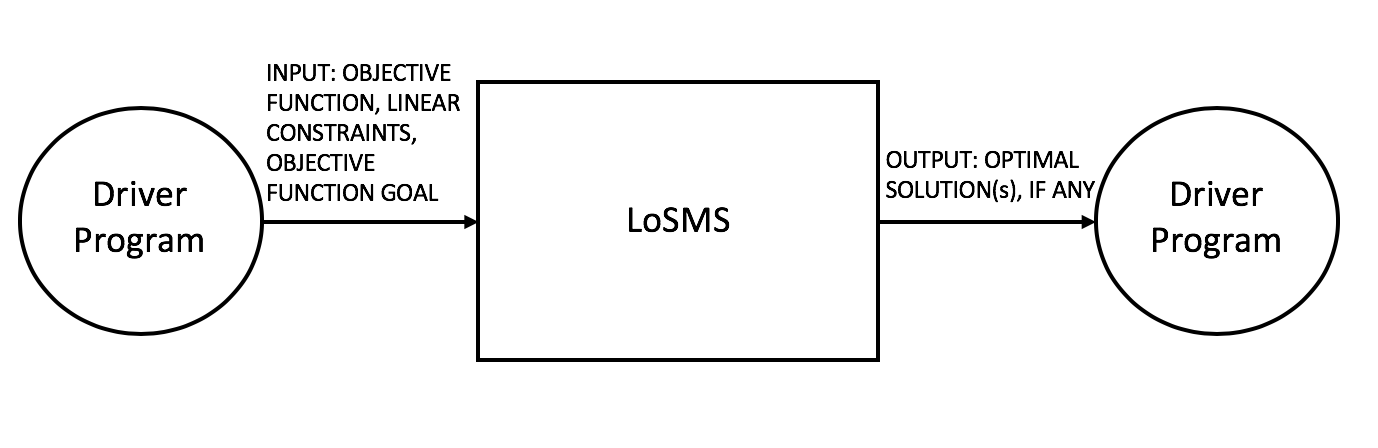
\includegraphics[width=0.9\textwidth, 
		height=0.20\textheight]{system-context}
		\caption{System Context}
		\label{Figure_SystemContext} 
	\end{center}
\end{figure}

Figure~\ref{Figure_SystemContext} describes the system context of \famname{}. 
The user inputs the correct data and \famname{} displays the output, if any.

\begin{itemize}
	\item User Responsibilities:
	\begin{itemize}
		\item Input the objective function, linear constraints and the 
		objective function goal.
	\end{itemize}
	\item \famname{} Responsibilities:
	\begin{itemize}
		\item Detect data type mismatch, such as a string of characters instead 
		of a floating point number.
		
		\item Handle any errors occuring when the user enters the inputs, such 
		as entering inputs in an incorrect format.
		
		\item Find and display the linear program's optimal solution(s) (if 
		any).
	\end{itemize}
\end{itemize}

\subsection{Potential User Characteristics} \label{SecUserCharacteristics}

The end user of \famname{} should have basic knowledge of linear programming  
which is typically given to year 3 undergraduate students.

\subsection{Potential System Constraints}

\famname{} does not have any system constraints.

\section{Commonalities} \label{Sec_Commonalities}

This section begins by providing a general idea about the \famname{} tool, 
followed by terminology and data definitions, goal statements and theoretical 
models.

\subsection{Background Overview} \label{Sec_Background}

\famname{} is a program family that facilitates obtaining the optimal solution 
of linear programs given the objective function and linear constraints. The 
tool can be beneficial for users coming from various fields, including physics 
and chemistry.

\subsection{Terminology and  Definitions}

This subsection provides a list of terms that are used in the subsequent
sections and their meaning, with the purpose of reducing ambiguity and making it
easier to correctly understand the requirements:

\begin{itemize}
	\item Linear program: An optimization problem where the goal is to minimize 
	or maximize the objective function.
	
	\item Objective function: The function to be minimized or maximized.
	
	\item Decision variables: ${x_1}$, ${x_2}$, ..., ${x_n}$
	
	\item Feasible solution: The point that satisfies all constraints and sign 
	restrictions.
	
	\item Feasible region: The set of all feasible points.
	
	\item Optimal solution/The optimum: A feasible solution with the maximum 
	value in maximization objective functions or the minimum value in 
	minimization objective functions.
\end{itemize}

\subsection{Data Definitions} \label{sec_datadef}

This section collects and defines all the data needed to build the instance
models. The dimension of each quantity is also given.  
	
~\newline

\noindent
\begin{minipage}{\textwidth}
	\renewcommand*{\arraystretch}{1.5}
	\begin{tabular}{| p{\colAwidth} | p{\colBwidth}|}
		\hline
		\rowcolor[gray]{0.9}
		Number& DD\refstepcounter{datadefnum}\thedatadefnum 
		\label{minToMax}\\
		\hline
		Label& \bf The Negation of a Minimization Linear Program\\
		\hline
		Symbol & $Z'$\\
		\hline
		Equation& $Z' = -Z$\\
		\hline
		Description & 
		To convert the linear program goal from minimization to maximization, 
		negate the minimization function by multiplying it by -1.
		\\
		\hline
		Sources& -\\
		\hline
		Ref.\ By & \iref{minLP}\\
		\hline
	\end{tabular}
\end{minipage}\\

~\newline

\noindent
\begin{minipage}{\textwidth}
	\renewcommand*{\arraystretch}{1.5}
	\begin{tabular}{| p{\colAwidth} | p{\colBwidth}|}
		\hline
		\rowcolor[gray]{0.9}
		Number& DD\refstepcounter{datadefnum}\thedatadefnum 
		\label{simplexTableau}\\
		\hline
		Label& \bf The Simplex Tableau\\
		\hline
		Symbol & - \\
		\hline
		Equation& $\begin{bmatrix}
		a_{11} & a_{12} & a_{13} & \dots & b_{1}\\
		a_{21} & a_{22} & a_{23} & \dots & b_{2}\\
		\vdots & \vdots & \vdots & &\vdots\\
		\vdots & \vdots & \vdots & &\vdots\\
		a_{n1} & a_{n2} & a_{n3} & \dots & b_{m}	
		\end{bmatrix}$ \\
		\hline
		Description & 
		The simplex tableau is the augmented matrix of the linear program's 
		equations.\\
		\hline
		Sources& -\\
		\hline
		Ref.\ By & \iref{maxLP}\\
		\hline
	\end{tabular}
\end{minipage}\\

~\newline

\noindent
\begin{minipage}{\textwidth}
	\renewcommand*{\arraystretch}{1.5}
	\begin{tabular}{| p{\colAwidth} | p{\colBwidth}|}
		\hline
		\rowcolor[gray]{0.9}
		Number& DD\refstepcounter{datadefnum}\thedatadefnum 
		\label{slackVar}\\
		\hline
		Label& \bf The Slack Variable\\
		\hline
		Symbol & $S_n$\\
		\hline
		Equation& $a_1x_1 + a_2x_2\;{\leq}\;b_m$ becomes $a_1x_1 + a_2x_2 + S_n 
		= b_m$ \\
		\hline
		Description & 
		The slack variable is a non-negative variable that is added to less 
		than or equal to inequalities so they become equalities.
		\\
		\hline
		Sources& \cite{lp-defs}\\
		\hline
		Ref.\ By & \iref{maxLP}, \aref{A_nonnegative}\\
		\hline
	\end{tabular}
\end{minipage}\\

\subsection{Goal Statements}

\noindent Given the objective function, linear constraints and the objective 
function goal, the goal statement of \famname{} is: 

\begin{itemize}
	\item[GS\refstepcounter{goalnum}\thegoalnum \label{goalStatement}:] Use the 
	simplex method to find and display the objective function's optimal 
	solution(s) satisfying all linear constraints and sign restrictions.
\end{itemize}

\subsection{Theoretical Models} \label{sec_theoretical}

This section focuses on the general equations and laws that \famname{} is based
on.

~\newline

\noindent
\begin{minipage}{\textwidth}
	\renewcommand*{\arraystretch}{1.5}
	\begin{tabular}{| p{\colAwidth} | p{\colBwidth}|}
		\hline
		\rowcolor[gray]{0.9}
		Number& T\refstepcounter{theorynum}\thetheorynum \label{T_LPSF}\\
	  	\hline
	  	Label&\bf The Standard Form of a Linear Program\\
	  	\hline
	  	Equation&\[
		  \left\{ \begin{array}{c}
		  max\;Z=\;\;\;c_{1}x_1 + c_{2}x_2 + ........ + c_{n}x_n \\ 
		  s.\;t.\;\;\;\; a_{11}x_1 + a_{12}x_2 + ........ + 
		  a_{1n}x_n\;{\leq}\;b_1 
		  \\
		  \hspace{1.3cm}\vdots \hspace{1.2cm}\vdots \hspace{2.6cm}\vdots 
		  \hspace{1.5cm}\vdots \\
		  \;\;\;\;\;\;\;\;\; a_{m1}x_1 + a_{m2}x_2 + ........ + 
		  a_{mn}x_n\;{\leq}\;b_m 
		  \\
		  x_1, x_2 + ........ + x_n\;{\geq}\;0 \\
		  \end{array}
		  \right. 
		  \]\\
	  	\hline
	  	Description & 
	      A linear program is in its standard form when it satisfies the 
	      following 
	      conditions: \newline
	      \begin{itemize}
	      	\item The objective function is a maximization function
	        
	        \item All constraints are inequalities
	        
	        \item All decision variables are non-negative
	      \end{itemize}\\
	  	\hline
	  	Source & \cite{lp-defs}\\
	  	\hline
	  	Ref.\ By & \iref{maxLP}, \rref{R_StandardForm}\\
	  	\hline
	\end{tabular}
\end{minipage}\\

~\newline

\noindent
\begin{minipage}{\textwidth}
	\renewcommand*{\arraystretch}{1.5}
	\begin{tabular}{| p{\colAwidth} | p{\colBwidth}|}
		\hline
		\rowcolor[gray]{0.9}
		Number& T\refstepcounter{theorynum}\thetheorynum \label{T_SLPCF}\\
		\hline
		Label&\bf The Canonical Form of a Standard Linear Program\\
		\hline
		Equation&\[
		\left\{ 
		\begin{array}{c}
		max\;Z=\;\;\;c_{1}x_1 + c_{2}x_2 + ........ + c_{n}x_n \\ 
		s.\;t.\;\;\;\; a_{11}x_1 + a_{12}x_2 + ........ + 
		a_{1n}x_n\;=\;b_1 \\
		\hspace{1.3cm}\vdots \hspace{1.2cm}\vdots 
		\hspace{2.6cm}\vdots \hspace{1.5cm}\vdots \\
		\;\;\;\;\;\;\;\;\; a_{m1}x_1 + a_{m2}x_2 + ........ + 
		a_{mn}x_n\;=\;b_m \\
		x_1, x_2 + ........ + x_n\;{\geq}\;0 \\
		\end{array}
		\right. 
		\]\\
		\hline
		Description & 
		A standard linear program is in its canonical form when it satisfies 
		the conditions in \tref{T_LPSF}, except: \newline
		\begin{itemize}
			\item The constraints must be equality constraints and not 
			inequalities
		\end{itemize}\\
		\hline
		Source & \cite{lp-defs}\\
		\hline
		Ref.\ By & \iref{maxLP}, \rref{R_CanonicalForm}\\
		\hline
	\end{tabular}
\end{minipage}\\

~\newline

\noindent
\begin{minipage}{\textwidth}
	\renewcommand*{\arraystretch}{1.5}
	\begin{tabular}{| p{\colAwidth} | p{\colBwidth}|}
		\hline
		\rowcolor[gray]{0.9}
		Number& T\refstepcounter{theorynum}\thetheorynum \label{T_pivoting}\\
		\hline
		Label&\bf Pivoting in an Augmented Matrix\\
		\hline
		Equation&$\begin{bmatrix}
		a_{11} & a_{12} & a_{13} & \dots & b_{1}\\
		\vdots & \vdots & \vdots & &\vdots\\
		a_{n1} & a_{n2} & a_{n3} & \dots & b_{m}	
		\end{bmatrix}$ \newline \newline
		Let $R_1$ = the first row in the matrix ; $R_n$ = the $n^{th}$ row in 
		the matrix: \newline
		Pivoting includes one or more of the following operations: \newline
		\begin{itemize}
			\item Row switching: $R_1 \xleftrightarrow{} R_n$
			
			\item Row addition: $R_1$ + $R_n$
			
			\item Multiplying a row by a non-zero constant: $aR_n$ ; 
			$a \neq 0$
		\end{itemize} \\
		\hline
		Description & 
		Pivoting in an augmented matrix consists of a series of row operations 
		that are done to clear a column in the matrix (set elements of the 
		column to zero).\\
		\hline
		Source & -\\
		\hline
		Ref.\ By & \iref{maxLP}\\
		\hline
	\end{tabular}
\end{minipage}\\

\section{Variabilities} \label{Sec_Variabilities} 

This section describes the variabilities in the \famname{} tool and details the 
instance models, assumptions and variabilities in the calculation and the 
output.

\subsection{Instance Models} \label{sec_instance}   

This section transforms the documented problem into one which is expressed in 
mathematical terms.

~\newline

\noindent
\begin{minipage}{\textwidth}
	\renewcommand*{\arraystretch}{1.5}
	\begin{tabular}{| p{\colAwidth} | p{\colBwidth}|}
		\hline
		\rowcolor[gray]{0.9}
		Number& IM\refstepcounter{instnum}\theinstnum \label{maxLP}\\
		\hline
		Label& \bf The Simplex Method for Solving Linear Programs: Maximization 
		Functions\\
		\hline
		Input& 
		\begin{enumerate}
			\item Max objective function: $max\;Z=\;c_{1}x_1 + c_{2}x_2 + ... + 
			c_{n}x_n$
			
			\item Linear constraint(s): 
			\newline$a_{m1}x_1 + a_{m2}x_2 + ... + a_{mn}x_n\;{\leq}\;b_m$
			\newline$x_1, ..., x_n\;{\geq}\;0$
		\end{enumerate}\\
		\hline
		Output& The optimal solution $Z$\\
		\hline
		Description& 
		\begin{enumerate}
			\item Convert linear program to its canonical form using slack 
			variables.
			
			\item Set up the simplex method tableau.
			
			\item Perform pivoting.
			
			\item Set up the new simplex tableau.
			
			\item Repeat steps 2-4 until there are no negative numbers in the 
			bottom row of the tableau.
			
			\item The optimal solution $Z$ is found in the basic feasible 
			solution derived from the final tableau.
		\end{enumerate}
		\\
		\hline
		Sources& \cite{lp-defs}\\
		\hline
		Ref.\ By & \iref{minLP}, \calcref{calculation}, \rref{R_Calculate}\\
		\hline
	\end{tabular}
\end{minipage}\\

~\newline

\noindent
\begin{minipage}{\textwidth}
	\renewcommand*{\arraystretch}{1.5}
	\begin{tabular}{| p{\colAwidth} | p{\colBwidth}|}
		\hline
		\rowcolor[gray]{0.9}
		Number& IM\refstepcounter{instnum}\theinstnum \label{minLP}\\
		\hline
		Label& \bf The Simplex Method for Solving Linear Programs: Minimization 
		Functions\\
		\hline
		Input& 
		\begin{enumerate}
			\item Min objective function: $min\;Z=\;c_{1}x_1 + c_{2}x_2 + ... + 
			c_{n}x_n$
			
			\item Linear constraint(s): 
			\newline$a_{m1}x_1 + a_{m2}x_2 + ... + a_{mn}x_n\;{\leq}\;b_m$
			\newline$x_1, ..., x_n\;{\geq}\;0$
		\end{enumerate}\\
		\hline
		Output& The optimal solution $Z$\\
		\hline
		Description& 
		\begin{enumerate}
			\item Convert the minimization linear program to a maximization 
			linear program.
			
			\item Solve \iref{maxLP}.
		\end{enumerate}
		\\
		\hline
		Sources& \cite{lp-defs}\\
		\hline
		Ref.\ By & \calcref{calculation}, \rref{R_Calculate} \\
		\hline
	\end{tabular}
\end{minipage}\\

\subsubsection*{Derivation of the Simplex Method}{
	The origin of the simplex method is detailed in \cite{simplex-origin}. 
}

\subsection{Assumptions}

\begin{itemize}
	\item[A\refstepcounter{assumpnum}\theassumpnum \label{A_nonnegative}:] The 
	 decision and slack variables are non-negative.
	
	\item[A\refstepcounter{assumpnum}\theassumpnum \label{A_inequalities}:] If 
	the linear constraints are inequalities, they are of type less than or 
	equal to. This is to ensure that all variables are non-negative.
\end{itemize}

\subsection{Calculation} \label{sec_Calculation}

\begin{itemize}
	\item[C\refstepcounter{calcnum}\thecalcnum \label{calculation}:] Solve 
	\iref{maxLP} for maximization problems and \iref{minLP} for minimization 
	problems.
\end{itemize}

\subsection{Output} \label{sec_Output}

All variabilities have the same output.    

\section{Requirements} \label{Sec_Requirements}

This section provides the functional requirements, the business tasks that the
software is expected to complete, and the nonfunctional requirements, the
qualities that the software is expected to exhibit.

\subsection{Functional Requirements}

\noindent 
\begin{itemize}
	\item[R\refstepcounter{reqnum}\thereqnum \label{R_Inputs}:] The \famname{} 
	tool shall read the objective function, linear constraints and the 
	objective function goal from the user.
	
	\item[R\refstepcounter{reqnum}\thereqnum \label{R_HandleInputErrors}:] The 
	\famname{} tool shall verify that all inputs are valid and satisfy 
	\aref{A_nonnegative} and \aref{A_inequalities}.
	
	\item[R\refstepcounter{reqnum}\thereqnum \label{R_DisplayErrorMsg}:] If 
	there are invalid inputs, the \famname{} tool shall display a corresponding 
	message to the user.
	
	\item[R\refstepcounter{reqnum}\thereqnum \label{R_StandardForm}:] The 
	\famname{} tool shall convert the objective function to its standard form 
	(\tref{T_LPSF}).
	
	\item[R\refstepcounter{reqnum}\thereqnum \label{R_CanonicalForm}:] The 
	\famname{} tool shall convert the standard objective function to its 
	canonical form (\tref{T_SLPCF}).

	\item[R\refstepcounter{reqnum}\thereqnum \label{R_Calculate}:] The 
	\famname{} tool shall find the optimal solution(s) of the linear program by 
	solving \iref{maxLP} or \iref{minLP}, depending on the objective function 
	goal.
	
	\item[R\refstepcounter{reqnum}\thereqnum \label{R_Output}:] The \famname{} 
	tool shall display the optimal solution(s) to the user, if any.
	
	\item[R\refstepcounter{reqnum}\thereqnum \label{R_OutputError}:] If the 
	given linear program does not have any optimal solutions, the \famname{} 
	tool shall display a corresponding message to the user.
\end{itemize}

\subsection{Nonfunctional Requirements}

\subsubsection*{Usability}

\noindent 
\begin{itemize}
	\item[NFR\refstepcounter{nfreqnum}\thenfreqnum \label{usability}:] It shall 
	take at most 10 minutes for the user to learn to use the \famname{} tool.
\end{itemize}

\subsubsection*{Robustness}

\begin{itemize}
	\item[NFR\refstepcounter{nfreqnum}\thenfreqnum \label{robustness}:] If the 
	\famname{} tool encounters an unexpected behavior, the tool shall display 
	a corresponding message to the user in no longer than 2 minutes.
\end{itemize}

\subsubsection*{Portability}

\begin{itemize}
	\item[NFR\refstepcounter{nfreqnum}\thenfreqnum \label{portability}:] The 
	\famname{} tool shall be operable in at least Windows and Mac platforms.
\end{itemize}

\section{Likely Changes} \label{Sec_LikelyChanges} 

\noindent 
\begin{itemize}
	\item[LC\refstepcounter{lcnum}\thelcnum\label{LC_inequalities}:] The 
	support for greater than or equal to inequalities in the linear constraints.
	
	\item[LC\refstepcounter{lcnum}\thelcnum\label{LC_moreAlgorithms}:] The 
	support for additional linear programming algorithms.
\end{itemize}

\section{Traceability Matrices and Graphs} \label{Sec_TraceabilityMatrix}

The purpose of a traceability matrix is to visualise the way different 
components of this CA are dependent on one another. Every time a component in a 
row is changed, the component in the corresponding column marked with an "X" 
may have to be changed as well.  Table~\ref{Table_traceability1} shows the 
traceability between the data definitions, theoretical models, instance models, 
assumptions and the calculation.

\begin{table}[h!]
	\centering
	\begin{tabular}{|c|c|c|c|c|c|c|c|c|c|c|c|}
		\hline        
		& \ddref{minToMax} & \ddref{simplexTableau} & \ddref{slackVar} & 
		\tref{T_LPSF} & \tref{T_SLPCF} & \tref{T_pivoting} & \iref{maxLP} & 
		\iref{minLP} & \aref{A_nonnegative} & \aref{A_inequalities} & 
		\calcref{calculation} \\
		\hline
		\ddref{minToMax} 	    &   &   &   &   &   &   &   & X &   &   &  \\
		\hline
		\ddref{simplexTableau}  &   &   &   &   &   &   & X &   &   &   &  \\ 
		\hline
		\ddref{slackVar} 		&   &   &   &   &   &   & X &   &   &   &  \\ 
		\hline
		\tref{T_LPSF} 		  	&   &   &   &   &   &   & X &   &   &   &  \\ 
		\hline
		\tref{T_SLPCF} 	  		&   &   &   &   &   &   & X &   &   &   &  \\ 
		\hline  
		\tref{T_pivoting} 		&   &   &   &   &   &   & X &   &   &   &  \\ 
		\hline
		\iref{maxLP} 	  		&   &   &   &   &   &   &   & X &   &   & X\\ 
		\hline
		\iref{minLP}   			&   &   &   &   &   &   &   &   &   &   & X\\ 
		\hline
		\aref{A_nonnegative}	&   &   &   &   &   &   & X &   &   &   &  \\
		\hline 
		\aref{A_inequalities} 	&   &   &   &   &   &   & X &   &   &   &  \\
		\hline
		\calcref{calculation} 	&   &   &   &   &   &   &   &   &   &   & \\
		\hline
	\end{tabular}
	\caption{Traceability Matrix Showing the Dependencies between Components of 
	this CA}
	\label{Table_traceability1}
\end{table}

\newpage

\bibliographystyle {plainnat}
\bibliography {../../refs/References}

\newpage

\section{Appendix}

	This section provides additional content related to this commonality 
	analysis.

\subsection{Symbolic Parameters}

There are no symbolic parameters used in this document.

\end{document}